%%%%%%%%%%%%%%%%%%%%%%%%%%%%%%%%
\section{Introduction}
\label{introduction}
%%%%%%%%%%%%%%%%%%%%%%%%%%%%%%%%

Independent component analysis (ICA) is similar in many aspects to principal component analysis (PCA). In PCA we look for an orthonormal base in which the data components are not
linearly dependent (uncorrelated), while in 
ICA we search for the coordinate system in which the components are independent. More precisely the aim of ICA is to transform the observed data $\X$ into maximally independent components $\S$ with use of an invertible linear transformation $W$, called the {\em transformation matrix}: $$
\S = W^T \X.
$$

Popular ICA methodology does not directly attempt to find components that are independent but rather components that are as non-Gaussian as possible.
This follows from the fact that one of the theoretical foundations of ICA is given by the dual view at the Central Limit Theorem \cite{hyvarinen2000independent}, which states that the distribution of the sum (average or linear combination) of $N$ independent random variables approaches Gaussian as  $N\rightarrow \infty$. Obviously if all source variables are Gaussian, the ICA method will not work. 

Another common approach to ICA based on the maximum likelihood estimation~\cite{pham1997blind} is recently gaining popularity \cite{hyvarinen2004independent,samworth2012independent,ICA2017pattern}.  Then we search for the optimally fitted to data cordinate system $B$ and marginal
densities $f_i$ such that the data density factors in base $B$ as the product of maringal densities. To obtain an efficient method and avoid 
overfitting we have to restrict the marginal densities $f_i$ to a class $\F$ of densities which has not too many parameters which can be easily estimated (clearly from obvious reasons this class has to be different from gaussians).  As $\F$ we typically choose the super-Gaussian logistic density or other heavy tails distributions.

In many applications of ICA we deal with the case when several sensors measure the latents variables and the rest of them record only the noise. This happens when the number of sources is unknown and may be less than the number of sensors (then we are looking for so-called {\em non-square mixing matrix} $W$).
Such a case is common for example in the identification of brain networks
in functional  magnetic resonance imaging (fMRI) 
\cite{beckmann2012modelling,green2002pca}.
%and then we are looking for so-called non-square mixing matrix.
In practice, most approaches deal with this problem by first applying PCA to the observations prior to classic ICA (PCA+ICA) to meet the assumption of square mixing and to reduce computational costs \cite{hyvarinen2004independent}. Although numerically effective, this approach may fail as it is not invariant with respect to linear transformation, since PCA will find a ``noise'' component if
it is sufficiently large. 

%\begin{landscape}
\begin{figure*}[t]
% ensure that we have normalsize text
\normalsize
\begin{center}
\subfigure[Original images 42049 and 220075.] {\label{fig:image_ICA_int_1}
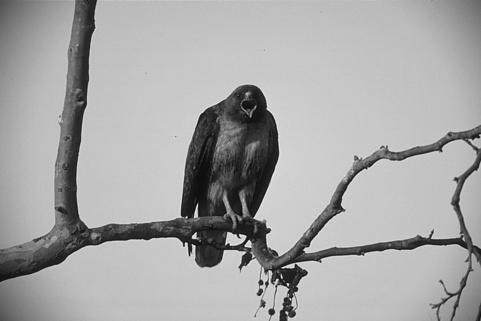
\includegraphics[width=1.6in]{2/2_6_or_1} 
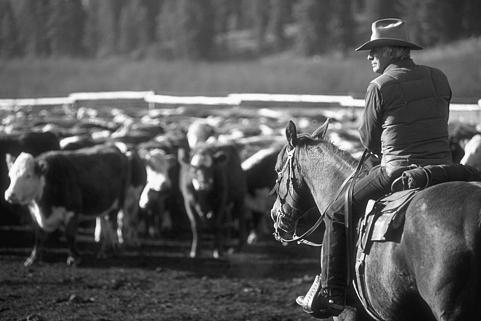
\includegraphics[width=1.6in]{2/2_6_or_2}
}
%%%%%%%%%%%%%%%%%%%%
%\subfigure[Sum and subtraction of images.] {\label{fig:image_ICA_int_2}
%\includegraphics[width=1.2in]{2/2_6_sum} 
%\includegraphics[width=1.2in]{2/2_6_div}
%} \\

%%%%%%%%%%%%%%%%%%%%
\subfigure[\ICA.] {\label{fig:image_ICA_int_3}
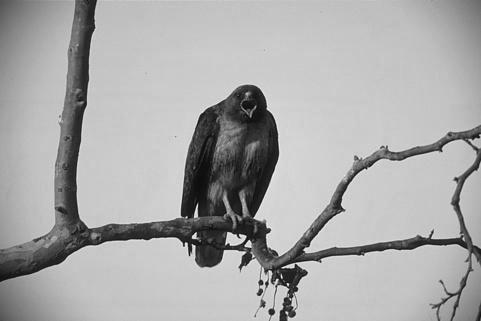
\includegraphics[width=1.6in]{2/2_6_ICA_FEW_II_2} 
}
\subfigure[FastICA.] {\label{fig:image_ICA_int_4}
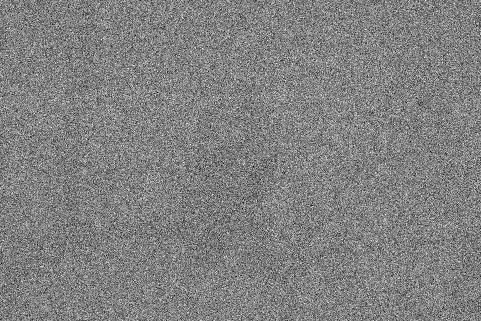
\includegraphics[width=1.6in]{2/2_6_ICA11_2} 
}
\subfigure[ProDenICA.] {\label{fig:image_ICA_int_5}
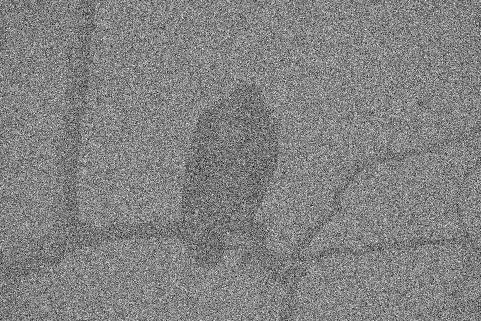
\includegraphics[width=1.6in]{2/2_6_ICA5_2} 
}\\
%%%%%%%%%%%%%%%%%%%%
\subfigure[\ICA.] {\label{fig:image_ICA_int_6}
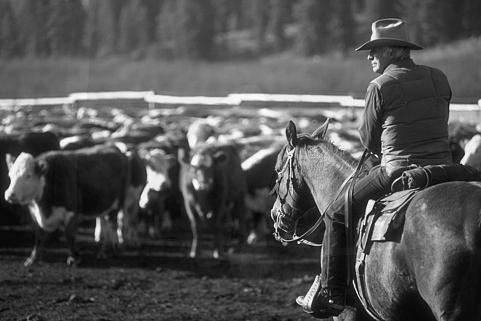
\includegraphics[width=1.6in]{2/2_6_ICA_FEW_II_1}
}
\subfigure[FastICA.] {\label{fig:image_ICA_int_7}
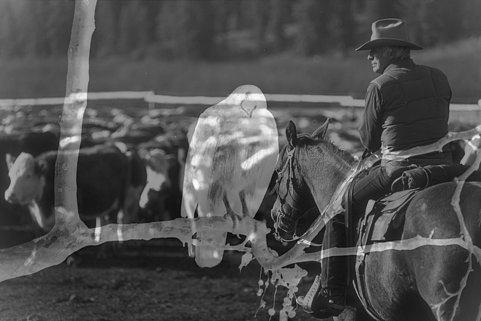
\includegraphics[width=1.6in]{2/2_6_ICA11_1}
}
\subfigure[ProDenICA.] {\label{fig:image_ICA_int_8}
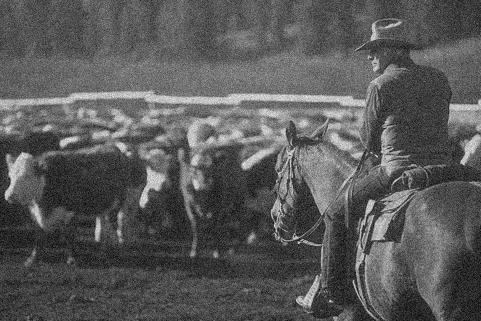
\includegraphics[width=1.6in]{2/2_6_ICA5_1}
}
\end{center}
\caption{Comparison of images separation by our method (\ICA), with FastICA and ProDenICA. Before mixing by a linear matrix, we added to the first two components given in (a) the third component given by random
normal noise. As we see \ICA{} was able to perfectly recover the two first components.}
\label{fig:image_ICA_int}
\end{figure*}

The aim of this paper is to propose a new density based approach to deal with this case which does not have the above
mentioned disadvantage. Our idea is to join the two earlier mentioned approaches to solving ICA - one based on the search for non-gaussian components and the
other based on density estimation - to deal with the case when the number of sources is smaller then that of sensors.  
Observe that the noise typically occurs as a sum of many independent
factors, and consequently thanks to the central limit theorem it typically has approximately gaussian distribution. This is why
one typically makes the assumption \cite{cover2012elements} that
$$
\text{\em noise components are comming from a gaussian noise.}
$$ 
Following the density approach to filter them out we fit the first $d$-components from a class of $\F$ of densities which is broader then gaussians, while the rest from the gaussians $\nor$ (the final choice of the value of parameter $d \in \{1,\ldots,D\}$ can be decided by applying either AIC or BIC criterion). Following \cite{ICA2017pattern} as $\F$ we take the class \SN{} of split-normal densities.

Our experiments show, which is illustrated by Figure \ref{fig:image_ICA_int}, that \ICA{} works as desired and effectively removes the components which contains gaussian noise. However, we cannot objectively conclude that it is better as compared to other state-of-the-art approaches, since the experiment 
was conducted in the setting optimal to our method as we assumed
that the noise was gaussian.
